\documentclass{article}

\usepackage{verbatim}
\usepackage{amsmath,amsfonts}
\usepackage{enumerate}
\usepackage{fancyvrb}

\newcommand{\ds}{\ensuremath{\displaystyle}}
\newcommand{\floor}[1]{\ensuremath{\left\lfloor#1\right\rfloor}}
\newcommand{\fracpart}[1]{\ensuremath{\left\{#1\right\}}}

\title{Intermediate Test 4}
\author{Stellenbosch Camp 2018}
\date{Time: $2\frac{1}{2}$ hours}


\begin{document}

\maketitle

\begin{enumerate}[1.]

\item % The Phil
How many numbers from $1$ to $2018$ inclusive can be written as the difference of two perfect squares?


\vspace{12pt}
\item %
Solve for $x$ and $y$. 

\begin{figure}[H]
\centering
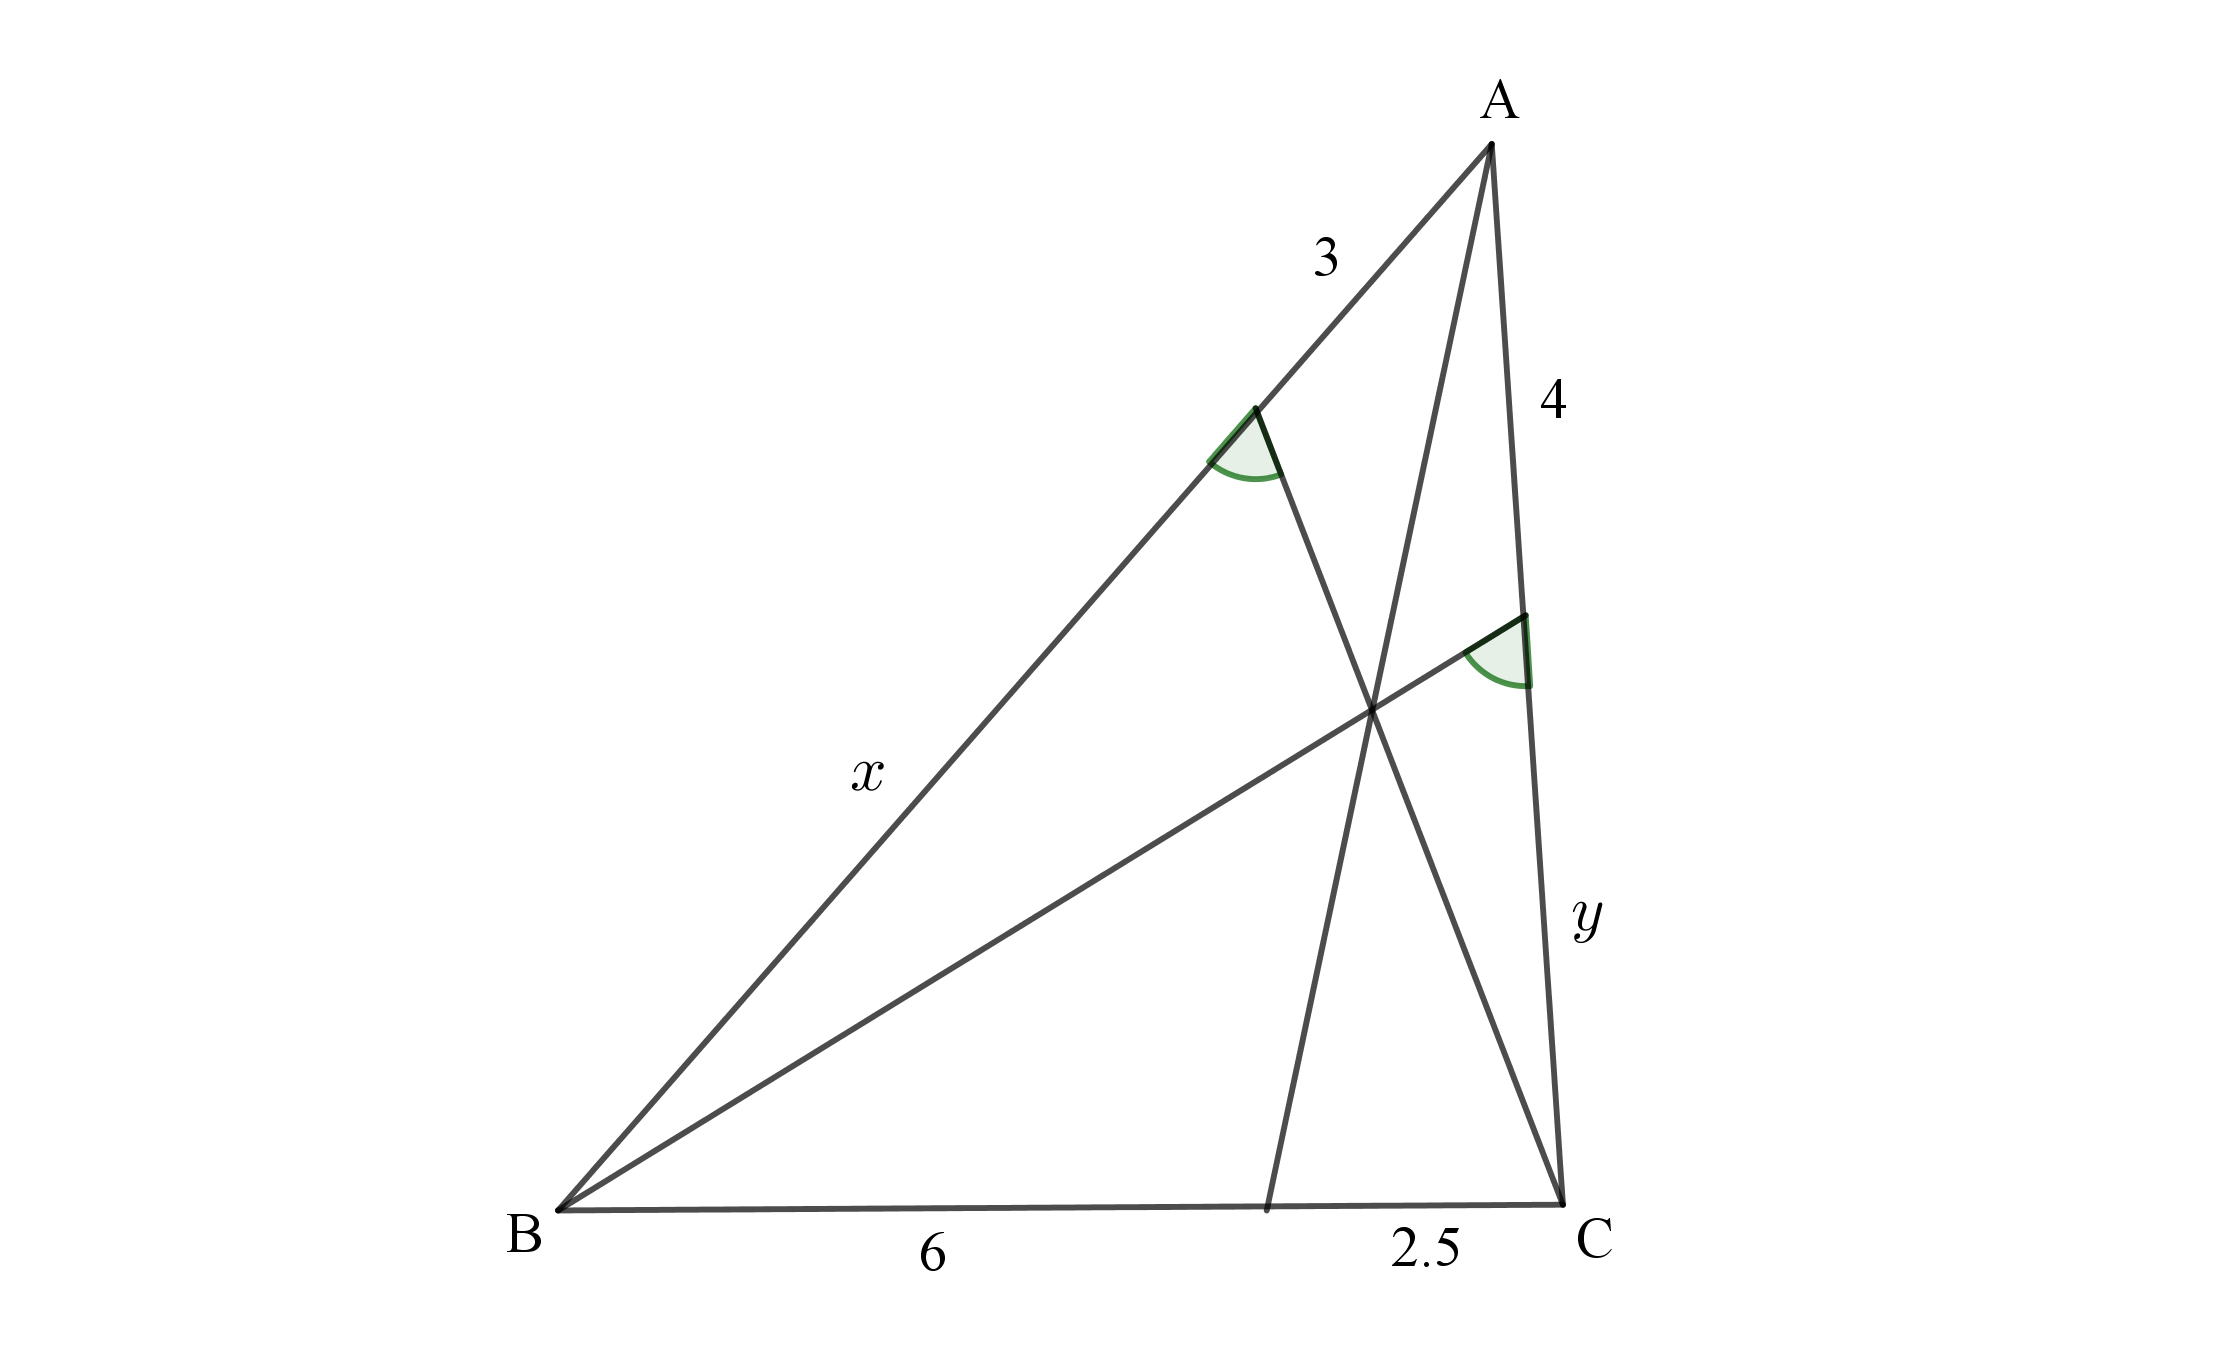
\includegraphics[width=0.9\linewidth]{GeogebraTest4.png}
\end{figure}


\vspace{12pt}
\item % The Dylan
Find all functions $f : \mathbb{R} -> \mathbb{R}$ such that for all real numbers $x$, \[ 2 f(x) +3 f(1-x) = x-4x^3. \]


\vspace{12pt}
\item % AoPS:  https://artofproblemsolving.com/community/c6t309f6h455752_integers_in_infinite_chessboard
Prove that it is impossible to write a positive integer in every cell of an infinite chessboard, in such a manner that, for all positive integers $m, n$, the sum of numbers in every $m\times n$ rectangle is divisible by $m + n$.


\vspace{12pt}
\item % Estonia 2007
An exam with $k$ questions is presented to $n$ students. A student fails the exam if they get less than half the answers right. We say that a question is easy if more than half of the students get it right. Decide if it is possible that

\begin{enumerate}
    \item[(a)]  All students fail even though all the questions were easy.
    \item[(b)] No student fails even though no question was easy.
\end{enumerate}


\end{enumerate}


\vfill
\centering
\begin{BVerbatim}
             .--~~,__
:-....,-------`~~'._.'
 `-,,,  ,_      ;'~U'
  _,-' ,'`-__; '--.
 (_/'~~      ''''(;
\end{BVerbatim}

\end{document}
